\documentclass{classrep}
\usepackage[utf8]{inputenc}
\frenchspacing

\usepackage{graphicx}
\usepackage[usenames,dvipsnames]{color}
\usepackage[hidelinks]{hyperref}
\usepackage{float}
\usepackage[table,xcdraw]{xcolor}
\usepackage{multirow}

\usepackage{amsmath, amssymb, mathtools}

\usepackage{fancyhdr, lastpage}
\pagestyle{fancyplain}
\fancyhf{}
\renewcommand{\headrulewidth}{0pt}
\cfoot{\thepage\ / \pageref*{LastPage}}

\renewcommand{\refname}{Bibliografia}

% bullet itemize
\renewcommand{\labelitemi}{\textbullet}

\studycycle{Informatyka stosowana, studia dzienne, II st.}
\coursesemester{2}

\coursename{Przetwarzanie i analiza dużych zbiorów danych}
\courseyear{2020/21}

\courseteacher{mgr inż. Rafał Woźniak}
\coursegroup{środa, 11:45}

\author{%
\\
  \studentinfo[234128@edu.p.lodz.pl]{Piotr Wardęcki}{234128}\\
  \studentinfo[234053@edu.p.lodz.pl]{Paweł Galewicz}{234053}\\
  \studentinfo[234067@edu.p.lodz.pl]{Bartosz Jurczewski}{234067}%
}

\title{Zadanie 3}

\begin{document}
\maketitle
\thispagestyle{fancyplain}
\clearpage

\section{Cel zadania}

Celem zadania była implementacja algorytmu \textit{k}-średnich z uwzględnieniem dwóch miar - Euklidesowej oraz Manhattan - dla dwóch sposobów generowania centrów - losowego oraz maksymalnie oddalonych od siebie punktów (według odległości euklidesowej). 

Dla każdej iteracji należało obliczyć funkcje kosztu $\phi(i)$ oraz $\psi(i)$, wygenerować wykresy oraz obliczyć procentową zmianę kosztu po 10 iteracjach algorytmu dla obydwu miar odległości z wskazaniem, które z dwóch początkowych rozmieszeń skupień pozwoliło uzyskać lepsze rezultaty.

Miara euklidesowa:
\begin{equation}
    \text{odległość:  } || a - b || = \sqrt{\sum_{i=1}^{d} (a_{i} - b_{i}) ^ 2 }
\end{equation}

\begin{equation}
    \text{koszt:  } \phi = \sum_{x \epsilon X} \min_{c \epsilon C} || x - c || ^ 2
\end{equation}

Miara Manhattan:
\begin{equation}
    \text{odległość:  } | a - b | = \sum_{i=1}^{d} | a_{i} - b_{i} |
\end{equation}

\begin{equation}
    \text{koszt:  } \psi =  \sum_{x \epsilon X} \min_{c \epsilon C} | x - c |
\end{equation}

%%%%%%%%%%%%%%%%%%%%%%%%%%%%%%%%%%%%%%%%%%%%  OPIS IMPLEMENTACJI
\section{Opis implementacji}
Do wykonywania zadania niezbędna była instancji \textit{Apache Spark}. Aby ograniczyć liczbę zainstalowanych środowisk skorzystaliśmy z odpowiedniego obrazu dla Dockera \cite{docker}, który zawierał także \textit{Jupyter Notebook}, \textit{Python} oraz \textit{Miniconda}. Dodatkowo aby ułatwić tworzenie środowiska do kolejnych zadań i między naszymi komputerami skorzystaliśmy z narzędzia \textit{Docker Compose} (nasz plik \cite{docker-compose}).

%%%%%%%%%%%%%%%%%%%%%%%%%%%%%%%%%%%%%%%%%%%%  WYNIKI
\section{Wyniki}

\begin{table}[H]
\centering
\caption{Uzyskane wartości funkcji kosztu}
\label{tab:res1}
\begin{tabular}{|c|c|c|c|c|}
\hline
\multirow{2}{*}{\textbf{Iteracja}} & \multicolumn{2}{c|}{\textbf{Metryka euklidesowa}} & \multicolumn{2}{c|}{\textbf{Metryka Manhattan}} \\ \cline{2-5} 
 & Plik 3b.txt & Plik 3c.txt & Plik 3b.txt & Plik 3b.txt \\ \hline
1 & 623660345.31 & 438747790.03 & 550117.14 & 1433739.31 \\ \hline
2 & 509862908.30 & 249803933.63 & 464869.28 & 1084488.78 \\ \hline
3 & 485480681.87 & 194494814.41 & 470897.38 & 973431.71 \\ \hline
4 & 463997011.69 & 169804841.45 & 483914.41 & 895934.59 \\ \hline
5 & 460969266.57 & 156295748.81 & 489216.07 & 865128.34 \\ \hline
6 & 460537847.98 & 149094208.11 & 487629.67 & 845846.65 \\ \hline
7 & 460313099.65 & 142508531.62 & 483711.92 & 827219.58 \\ \hline
8 & 460003523.89 & 132303869.41 & 475330.77 & 803590.35 \\ \hline
9 & 459570539.32 & 117170969.84 & 474871.24 & 756039.52 \\ \hline
10 & 459021103.34 & 108547377.18 & 457232.92 & 717332.90 \\ \hline
11 & 458490656.19 & 102237203.32 & 447494.39 & 694587.93 \\ \hline
12 & 457944232.59 & 98278015.75 & 450915.01 & 684444.50 \\ \hline
13 & 457558005.20 & 95630226.12 & 451250.37 & 674574.75 \\ \hline
14 & 457290136.35 & 93793314.05 & 451974.60 & 667409.47 \\ \hline
15 & 457050555.06 & 92377131.97 & 451570.36 & 663556.63 \\ \hline
16 & 456892235.62 & 91541606.25 & 452739.01 & 660162.78 \\ \hline
17 & 456703630.74 & 91045573.83 & 453082.73 & 656041.32 \\ \hline
18 & 456404203.02 & 90752240.10 & 450583.67 & 653036.75 \\ \hline
19 & 456177800.54 & 90470170.18 & 450368.75 & 651112.43 \\ \hline
20 & 455986871.03 & 90216416.18 & 449011.36 & 646481.16 \\ \hline
\end{tabular}
\end{table}

Zmianę względną oznaczyliśmy grecką literą $\Delta$.

\small{
\[ \Delta \phi_{3b.txt} \Big(  \phi_{3b.txt}(1), \phi_{3b.txt}(10) \Big) = \frac{623 660 345,31 - 459 021 103,34}{623 660 345,31} = 0,2639886329 \approx 26,4\% \] 
\[ \Delta \phi_{3c.txt} \Big(  \phi_{3c.txt}(1), \phi_{3c.txt}(10) \Big) = \frac{438 747 790,03 - 108 547 377,18}{438 747 790,03} = 0,7525973244 \approx 75,26\% \]
\[ \Delta \psi_{3b.txt} \Big(  \psi_{3b.txt}(1), \psi_{3b.txt}(10) \Big) = \frac{550 117,14 - 457 232,92}{550 117,14} = 0,1688444392 \approx 16,88\% \]
\[ \Delta \psi_{3c.txt} \Big(  \psi_{3c.txt}(1), \psi_{3c.txt}(10) \Big) = \frac{1 433 739,31 - 717 332,90}{1 433 739,31} = 0,4996768973 \approx 49,97\% \]
}
\subsection{Wykresy dla losowo wygenerowanych punktów}
\begin{figure}[H]
        \centering
        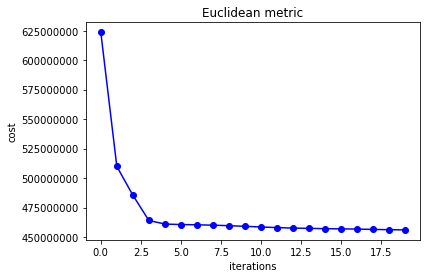
\includegraphics[width=1\textwidth]{images/images3/RandomEuclidean.png}
        \caption{Metryka Euklidesowa dla losowych punktów - 3b.txt}
        \label{fig1}
    \end{figure}
\begin{figure}[H]
        \centering
        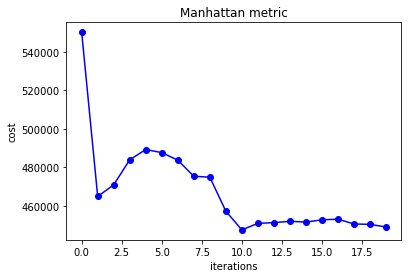
\includegraphics[width=1\textwidth]{images/images3/RandomManhattan.png}
        \caption{Metryka Manhattan dla losowych punktów - 3b.txt}
        \label{fig2}
    \end{figure}
\subsection{Wykresy dla punktów najbardziej oddalonych od siebie}

\begin{figure}[H]
        \centering
        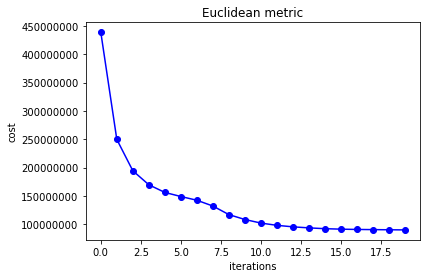
\includegraphics[width=1\textwidth]{images/images3/AwayEuclidean.png}
        \caption{Metryka Euklidesowa dla punktów oddalonych najdalej do siebie - 3c.txt}
        \label{fig3}
    \end{figure}
\begin{figure}[H]
        \centering
        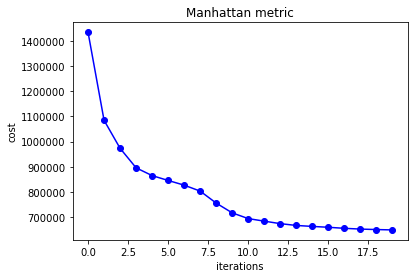
\includegraphics[width=1\textwidth]{images/images3/AwayManhattan.png}
        \caption{Metryka Manhattan dla punktów oddalonych najdalej do siebie - 3c.txt}
        \label{fig4}
    \end{figure}

%%%%%%%%%%%%%%%%%%%%%%%%%%%%%%%%%%%%%%%%%%%% Wnioski
\section{Wnioski}

\begin{itemize}
    \item Przy centrach wybieranych z najbardziej oddalonych od siebie punktów zmiana kosztu w kolejnych iteracjach jest znacząco większa niż w przypadku punktów losowych. Jest to spowodowane tym, że w pierwszych kilku iteracjach centra będą znajdowały się na "krańcach" zbioru danych, dlatego odległości od punktów są bardzo duże.
    \item Dla losowo wybranych centrów metryka Euklidesowa wydaje się być bardziej optymalna. Kosz pierwszej iteracji jest mniejszy, niż koszt 20 iteracji przy najbardziej oddalonych punktach. 
    \item Odwrotnie jest w przypadku metryki Manhattan. Tutaj lepszą metodą wydaje się branie najbardziej oddalonych punktów.
    \item Przypadek \ref{fig2} jest jedynym, w który występuje wzrost kosztu w kilku kolejnych iteracjach. Anomalia ta może wynikać z niekorzystnego doboru losowych punktów wybranych na centra.
    \item \textit{Apache Spark} jest szczególnie przydatny do równoległego przetwarzania rozproszonych danych za pomocą algorytmów iteracyjnych.

\end{itemize}

% \newpage

\nocite{*}
\begin{thebibliography}{0}
    
    \bibitem{docker}
    \textsl{Jupyter Notebook Python, Spark Stack}
    \url{https://hub.docker.com/r/jupyter/pyspark-notebook}

    \bibitem{docker-compose}
    \textsl{Plik Docker Compose do zadania 2}
    \url{https://github.com/jurczewski/PiADZD/blob/master/zad2/docker-compose.yml}

    
\end{thebibliography}
\end{document}